\documentclass[./bab_3.tex]{subfiles}
\begin{document}
  \section{Pemodelan yang digunakan}
  \subsection{Topologi Jaringan}
  \paragraph*{}Pemodelan yang digunakan merepresentasikan
  susunan dari komputer yang ada pada jaringan. Pada
  perancangan jaringan yang akan diimplementasikan mitmproxy
  menggunakan pemodelan topologi jaringan.

  \begin{figure}[hbt!]
  \centering
    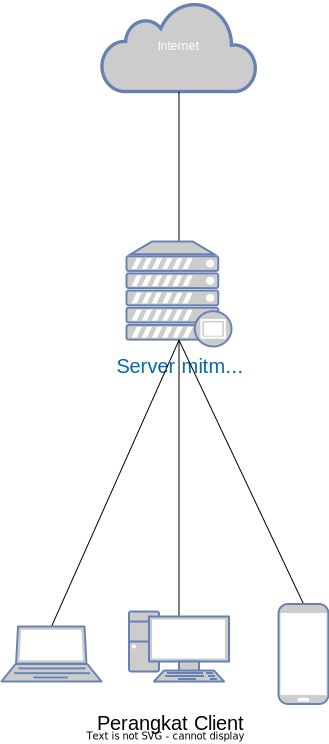
\includegraphics[scale=0.4]{topology01.png}
    \caption{Topologi Jaringan Sistem}
  \end{figure}

  \paragraph*{}Sistem yang dibuat merupakan server proxy, sehingga
  perangkat-perangkat client akan terhubung ke proxy
  terlebih dahulu sebelum terhubung pada internet.

  \subsection{Algoritma}
  \begin{figure}[hbt!]
  \centering
    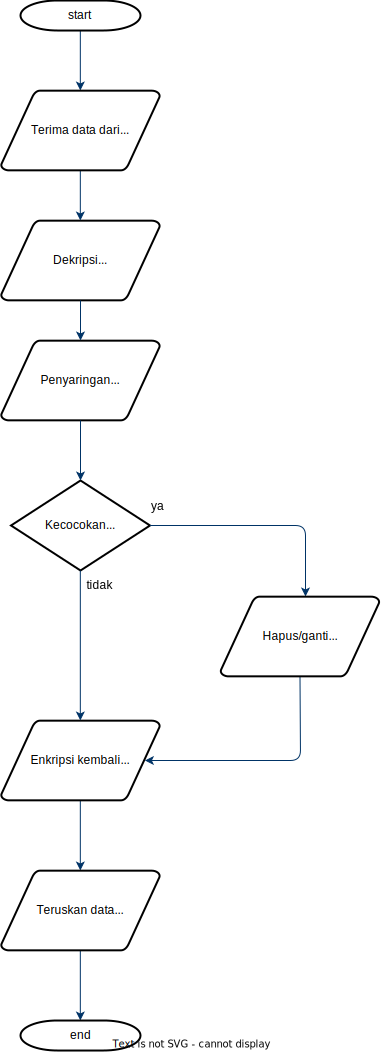
\includegraphics[scale=0.4]{flowchart01.png}
    \caption{Algoritma Sistem Mitmproxy}
  \end{figure}

  \paragraph*{}Untuk melakukan enkripsi diperlukan
  \textit{certificate}. \textit{Certificate} dapat diperoleh
  dari yang sudah dibuat oleh mitmproxy, atau dapat juga
  dibuat dengan menggunakan OpenSSL. Untuk membuat
  \textit{certificate} dengan menggunakan OpenSSL, Gunakan
  perintah:

  \mintinline[fontfamily=Courier New, fontsize=\normalsize]{bash}{openssl req -key private_key -x509 -new -days days -out namafile}

  Setelah \textit{certificate} didapatkan,
  \textit{certificate} tersebut perlu untuk diinstall di
  perangkat \textit{client}.

  \paragraph*{}Sedangkan untuk melakukan penyaringan konten,
  memanfaatkan \textit{library} Python BeautifulSoup dan
  library JSON \textit{built-in} di Python. \textit{Library}
  BeautifulSoup digunakan untuk mencari komponen-komponen
  HTML secara idiomatis, yang digunakan untuk menampilkan
  halaman web.
  Sedangkan library JSON digunakan untuk
  mem-\textit{parsing} data JSON, karena ada beberapa
  halaman web yang memanfaatkan FetchAPI untuk mengunduh
  kontennya. FetchAPI biasanya berkomunikasi dengan format
  data JSON. Dengan menggunakan \textit{library} ini
  diharapkan pembuatan script python untuk memfilter konten
  yang ditentukan menjadi mudah, karena tidak harus mencari
  komponen-komponen HTML dengan menuliskan
  \textit{regular-expression}.

\end{document}
